\chapter{Getting Started}

\section{Account Setup}

\subsection{Creating Your Account}

To begin using KanardiaCloud, you'll need to create an account:

\begin{enumerate}
    \item Navigate to the KanardiaCloud login page
    \item Click on the \textbf{"Register"} or \textbf{"Sign Up"} link
    \item Fill in the required information:
    \begin{itemize}
        \item Email address (must be valid)
        \item Full name
        \item Secure password
        \item Confirm password
    \end{itemize}
    \item Accept the Terms of Service and Privacy Policy
    \item Click \textbf{"Create Account"}
    \item Check your email for verification instructions
    \item Click the verification link to activate your account
\end{enumerate}

\begin{figure}[H]
\centering
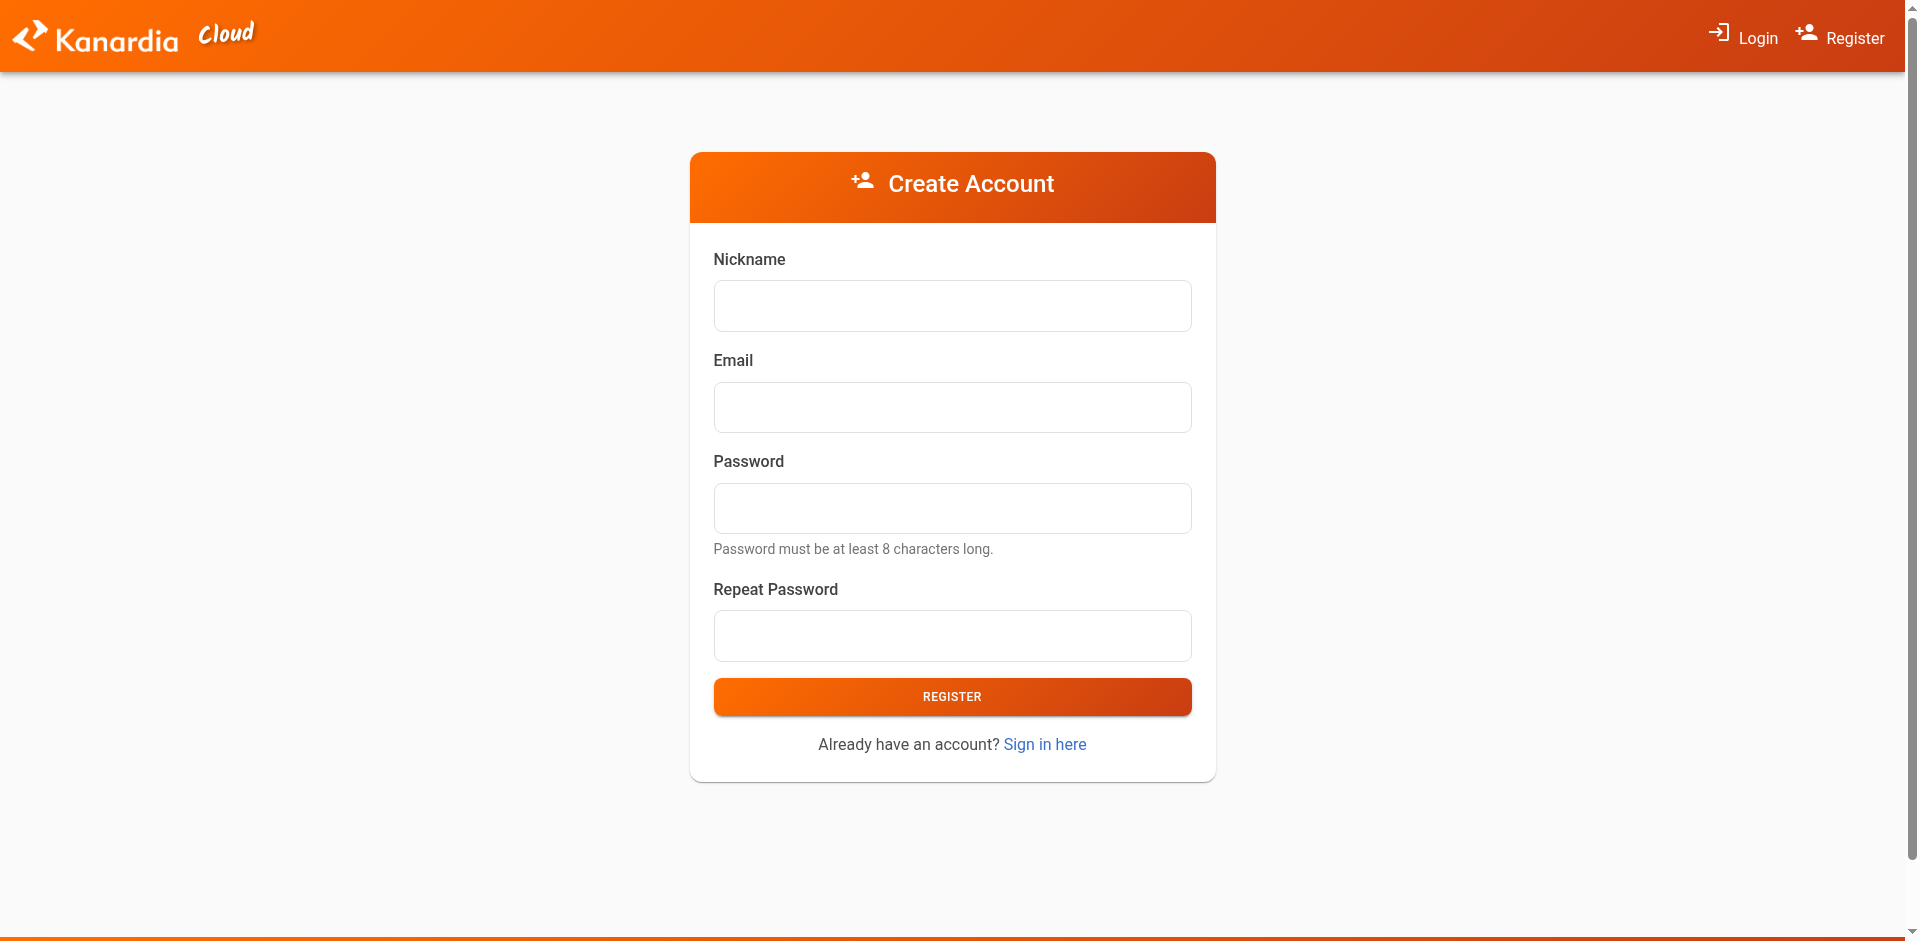
\includegraphics[width=0.8\textwidth]{images/registration_form.png}
\caption{Account Registration Form}
\label{fig:registration_form}
\end{figure}

\subsection{First Login}

After account verification:

\begin{enumerate}
    \item Return to the KanardiaCloud login page
    \item Enter your email address and password
    \item Click \textbf{"Sign In"}
    \item Complete the initial setup wizard (if prompted)
\end{enumerate}

\section{Dashboard Overview}

Upon successful login, you'll be greeted with the KanardiaCloud dashboard, which serves as your central command center.

\begin{figure}[H]
\centering
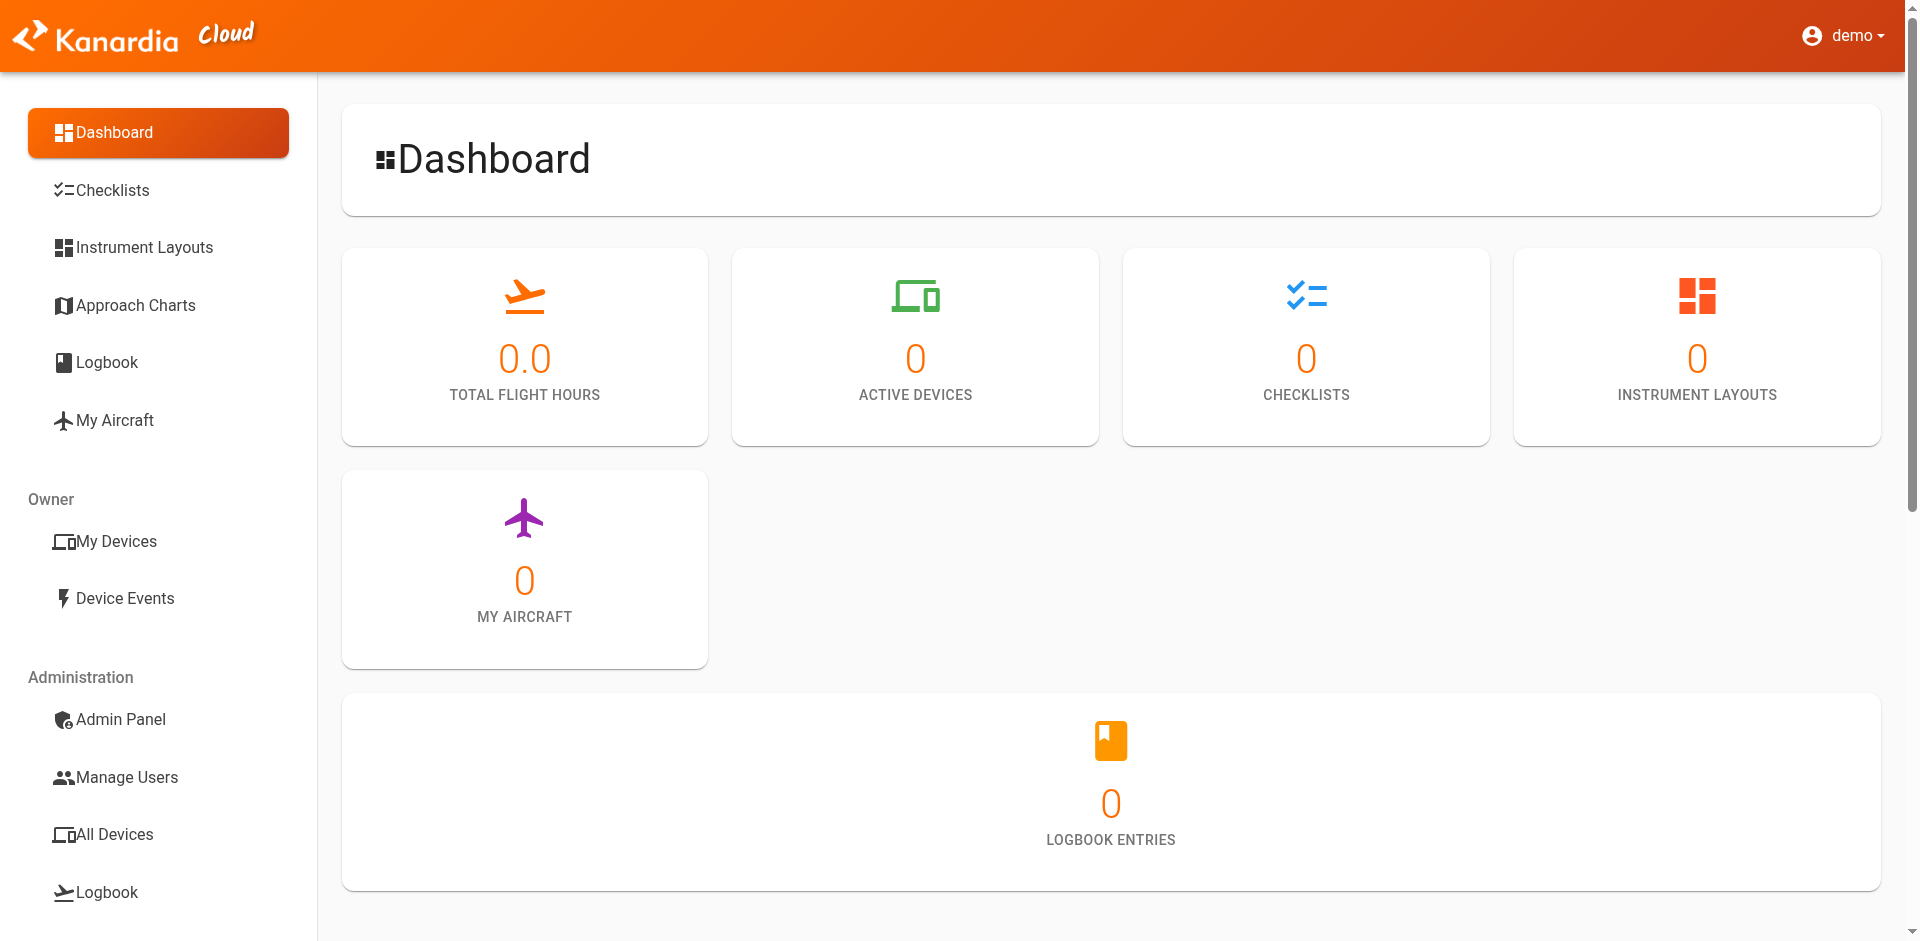
\includegraphics[width=\textwidth]{images/dashboard_overview.png}
\caption{KanardiaCloud Dashboard Overview}
\label{fig:dashboard_overview}
\end{figure}

\subsection{Navigation Menu}

The main navigation menu provides access to all KanardiaCloud features:

\begin{table}[H]
\centering
\begin{tabular}{@{}lp{8cm}@{}}
\toprule
\textbf{Menu Item} & \textbf{Description} \\
\midrule
Dashboard & Main overview with key metrics and recent activity \\
Devices & Manage and sync with Kanardia aviation devices \\
Checklists & Create, edit, and organize digital flight checklists \\
Instrument Layouts & Design custom instrument panel configurations \\
Logbook & Electronic flight logbook with automatic entries \\
Approach Charts & Store and manage airport approach procedures \\
Settings & User preferences and account configuration \\
\bottomrule
\end{tabular}
\caption{Main Navigation Menu Items}
\label{tab:navigation_menu}
\end{table}

\subsection{Quick Actions}

The dashboard provides quick access to common tasks:

\begin{itemize}
    \item \textbf{Add New Device}: Connect a new Kanardia device
    \item \textbf{Create Checklist}: Start building a new flight checklist
    \item \textbf{New Logbook Entry}: Manually add a flight record
    \item \textbf{Upload Chart}: Add new approach charts
\end{itemize}

\section{User Interface Elements}

\subsection{Common Controls}

KanardiaCloud uses consistent interface elements throughout the application:

\begin{description}
    \item[Primary Buttons] Orange buttons for main actions (Create, Save, Submit)
    \item[Secondary Buttons] Gray buttons for alternative actions (Cancel, Back)
    \item[Icon Buttons] Small buttons with icons for quick actions
    \item[Form Fields] Input fields with validation and error messages
    \item[Data Tables] Sortable and filterable tables for data display
\end{description}

\subsection{Status Indicators}

Various status indicators help you understand system states:

\begin{itemize}
    \item \textcolor{green}{\textbf{Green}}: Active, online, or successful states
    \item \textcolor{orange}{\textbf{Orange}}: Warning or attention required
    \item \textcolor{red}{\textbf{Red}}: Error, offline, or critical states
    \item \textcolor{gray}{\textbf{Gray}}: Inactive, disabled, or neutral states
\end{itemize}

\section{Basic Navigation}

\subsection{Moving Between Sections}

\begin{itemize}
    \item Use the main navigation menu on the left side
    \item Click the KanardiaCloud logo to return to the dashboard
    \item Use breadcrumb navigation for nested pages
    \item Browser back/forward buttons work as expected
\end{itemize}

\subsection{Searching and Filtering}

Most data views include search and filter capabilities:

\begin{enumerate}
    \item Look for the search box (usually in the top-right of data tables)
    \item Enter keywords to filter results in real-time
    \item Use dropdown filters for specific criteria
    \item Clear filters by clicking the "Clear" or "Reset" button
\end{enumerate}

\section{Getting Support}

\subsection{In-App Help}

\begin{itemize}
    \item Look for help icons (\texttt{?}) next to form fields
    \item Hover over tooltips for additional information
    \item Check the status bar for helpful hints
\end{itemize}

\subsection{Keyboard Shortcuts}

Common keyboard shortcuts available throughout the application:

\begin{table}[H]
\centering
\begin{tabular}{@{}ll@{}}
\toprule
\textbf{Shortcut} & \textbf{Action} \\
\midrule
Ctrl + S & Save current form or changes \\
Ctrl + N & Create new item (context-dependent) \\
Ctrl + F & Focus search field \\
Esc & Cancel current action or close modal \\
Tab & Navigate between form fields \\
\bottomrule
\end{tabular}
\caption{Keyboard Shortcuts}
\label{tab:keyboard_shortcuts}
\end{table}

\section{Initial Configuration}

\subsection{User Profile Setup}

Before using KanardiaCloud extensively, configure your user profile:

\begin{enumerate}
    \item Navigate to \textbf{Settings} $\rightarrow$ \textbf{User Profile}
    \item Update your personal information
    \item Set your preferred date/time format
    \item Configure notification preferences
    \item Set your default timezone
\end{enumerate}

\subsection{Device Connection}

If you have Kanardia devices to connect:

\begin{enumerate}
    \item Go to \textbf{Devices} section
    \item Click \textbf{"Add New Device"}
    \item Follow the device-specific setup wizard
    \item Test the connection
    \item Configure sync preferences
\end{enumerate}

\subsection{Data Import}

If you have existing flight data to import:

\begin{enumerate}
    \item Navigate to the appropriate section (Logbook, Checklists, etc.)
    \item Look for \textbf{"Import"} options
    \item Follow the import wizard
    \item Review and confirm imported data
\end{enumerate}
